%
% string matching writeup...
%

\documentclass{llncs}
\pagestyle{empty}
\usepackage{makeidx}  % allows for indexgeneration
%
\usepackage[dvips]{graphicx}    % needed for including graphics e.g. EPS, PS
\usepackage{epsfig}
\usepackage{url}
\usepackage{pseudocode}
\usepackage{comment}
\usepackage{authblk}
\usepackage{color}
\usepackage{newalg}
\usepackage{subfigure}

\begin{document}
\renewcommand{\labelenumi}{(\Alph{enumi})}
\renewcommand{\labelenumii}{(\alph{enumii})}

\frontmatter          % for the preliminaries
%
\pagestyle{headings}  % switches on printing of running heads

\mainmatter              % start of the contributions
%
\title{Bridging the gap: improving local multiple alignment with gapped extension.}
%
\titlerunning{procrastination for local multiple alignment}  % abbreviated title (for running head)
%                                     also used for the TOC unless
%                                     \toctitle is used
\author{...}

%\institute{ 
%Algorithms and Genetics Group, Dept. of Computer Science, Technical Univ. of Catalonia, Barcelona, Spain\\
%\email{treangen@lsi.upc.edu},\\
%}
%
\authorrunning{<Quijote> et al.}   % abbreviated author list (for running head)

\maketitle


\begin{abstract}
The identification of homologous DNA via sequence alignment is a basic building block in comparative genomics.  We present a method for accurately and sensitively identifying homologous DNA sequence in multiple genomes. Our method is based around an efficient heuristic for local multiple alignment, featuring a novel method for gapped extensions. In practice, we are able to sensitively identify conserved, potentially repetitive, regions in one or more DNA sequences.  The GPL implementation of our algorithm in C++ is
called \texttt{procrastAligner} and is freely available from
\url{http://gel.ahabs.wisc.edu/procrastination}
\end{abstract}




\section{ Introduction }

A central task in comparative genomics is being able to accurately identify all homologous positions in one or more DNA sequences. Local sequence alignment has traditionally considered to be the main tool for this task, and specifically, heuristics such as BLAST~\cite{...} and RepeatMasker~\cite{...} have been long employed for this exact purpose. Initially, the focus was on pairwise homology relationships, that is, finding all possible pairs of homologous regions in the input sequence(s). Pairwise local alignment can be used for orthology mapping~\cite{ref-orthomcl}, repeat detection~\cite{repseek}, and more~\cite{more}. More recently, partly due to the recent surge in available sequence data~\cite{...}, there has been a desire to expand pairwise relationships to multiple by grouping all pairwise homologous regions into groups(blocks,piles)~\cite{...}. Even so, homology detection methods based around pairwise local alignment have a tough time handling inconsistency issues when attempting to glue or merge all pairwise relationships. Also, highly repetitive regions in the input sequences can cause problems in efficiency, as they must conduct $O(n^{2})$ pairwise comparisons for each of the repeated regions. Highly repetitive ALU repeats and IS elements in microbes are just two common examples of the overwhelming abundance of repetitive sequence in genomes. 

However, instead of aligning each pair of the repeat, a single local multiple alignment can be constructed for all of the copies of the repeated sequence. Local multiple alignments can thus be used to identify the basic repeating units in one or more sequences, as well as serve as a basis for downstream analysis tasks such as multiple genome alignment~\cite{ref-mauve,ref-mga,ref-mgcat,ref-deweyReview}, global alignment with repeats~\cite{ref-otherSammethPaper,ref-aba}, or repeat classification and analysis~\cite{ref-piler}. Local multiple alignment also avoids dealing with consistency issues when try to resolve and merge boundaries of homology between all pairwise relationships. Finally, accuracy also benefits~\cite{...}cite a paper which shows multiple alignment is more accurate than pairwise alignment.  MUSCLE's iterative refinement procedure ensures
a high-scoring alignment irrespective of guide tree.

While lma offers many benefits over lpa, the cost of alignment in multiple sequences grows exponentially with respect to the number of sequences. Practically this means that we must find clever ways to perform and limit the amount of gapped alignment via dynamic programming that is performed in order to ensure efficiency. Gapped alignments arise when trying to extend seeds to fully capture surrounding sequence homology. Previous approaches have used X-drop~\cite{...} or related methods to reasonably limit this time consuming step. Our aim is to bridge this gap in efficiency by presenting a novel method for gapped extension for sensitive local multiple alignment.


%need for a new approach
%To date~\cite{gold}, there are over 500 completed whole genomes in such databases, and in the next few years this number is %expected to reach nearly 3000. To cope with such increases in data volume, corresponding advances in computational methods are %necessary; thus we present an efficient heuristic for local multiple alignment. Our method is based around an efficient %heuristic for local multiple alignment, featuring a novel method for gapped extensions.
\label{sec:overview}
\section{A heuristic for local multiple alignment}

Our heuristic approach to local multiple alignment
involves the following five steps:
\begin{description}
\item[Step 1:] Detect seeds in DNA sequence(s).
\item[Step 2:] Chain multi-matches
\item[Step 3:] Gapped extension of chains
\item[Step 4:] Define homology borders with random walk statistics
\item[Step 5:] Unalign non-homologous sequence
\end{description}

Before describing each step in more detail, we first need to define relevant terminology.
Given a sequence $\mathcal{S}=s_1, s_2,\dots, s_N$ of length $N$
defined over an alphabet $\{A,C,G,T\}$, our goal is to identify all homologous
local multiple alignments on subsequences of $\mathcal{S}$. We denote
an ungapped alignment, or match, among subsequences in $\mathcal{S}$
as an object $M$.  We refer the number of regions in $\mathcal{S}$
matched by a given match $M_i \in \mathbf{M}$ as the
\textit{multiplicity} of $M_i$, denoted as $|M_i|$.   We assume as input a set of ungapped alignments
$\mathbf{M}$.  We refer the number of regions in $\mathcal{S}$
matched by a given match $M_i \in \mathbf{M}$ as the
\textit{multiplicity} of $M_i$, denoted as $|M_i|$. When aligning DNA sequences, matches may
occur on the forward or reverse complement strands. To account for
this phenomenon we add an orientation value to each matching region 
where 1 indicates a forward strand match and -1 for reverse.

Our algorithm has an important limitation on the matches in
$\mathbf{M}$: no two matches $M_i$ and $M_j$ may have the same
left-end coordinate, e.g. $M_i.L_x \neq M_j.L_y~\forall~i, j, x, y$
except for the identity case when $i=j$ and $x=y$.  This constraint
has been referred to by others as \textit{consistency} and
\textit{transitivity}~\cite{ref-transitivity} of matches.  In the
present work we only require consistency and transitivity of matches
longer than the seed length, e.g. seed matches may overlap.

We denote a gapped alignment over an alphabet $\{A,C,G,T,-\}$ as $A$. 

\begin{figure}[t]
\begin{center}
\subfigure[Visual representation of our algorithm]{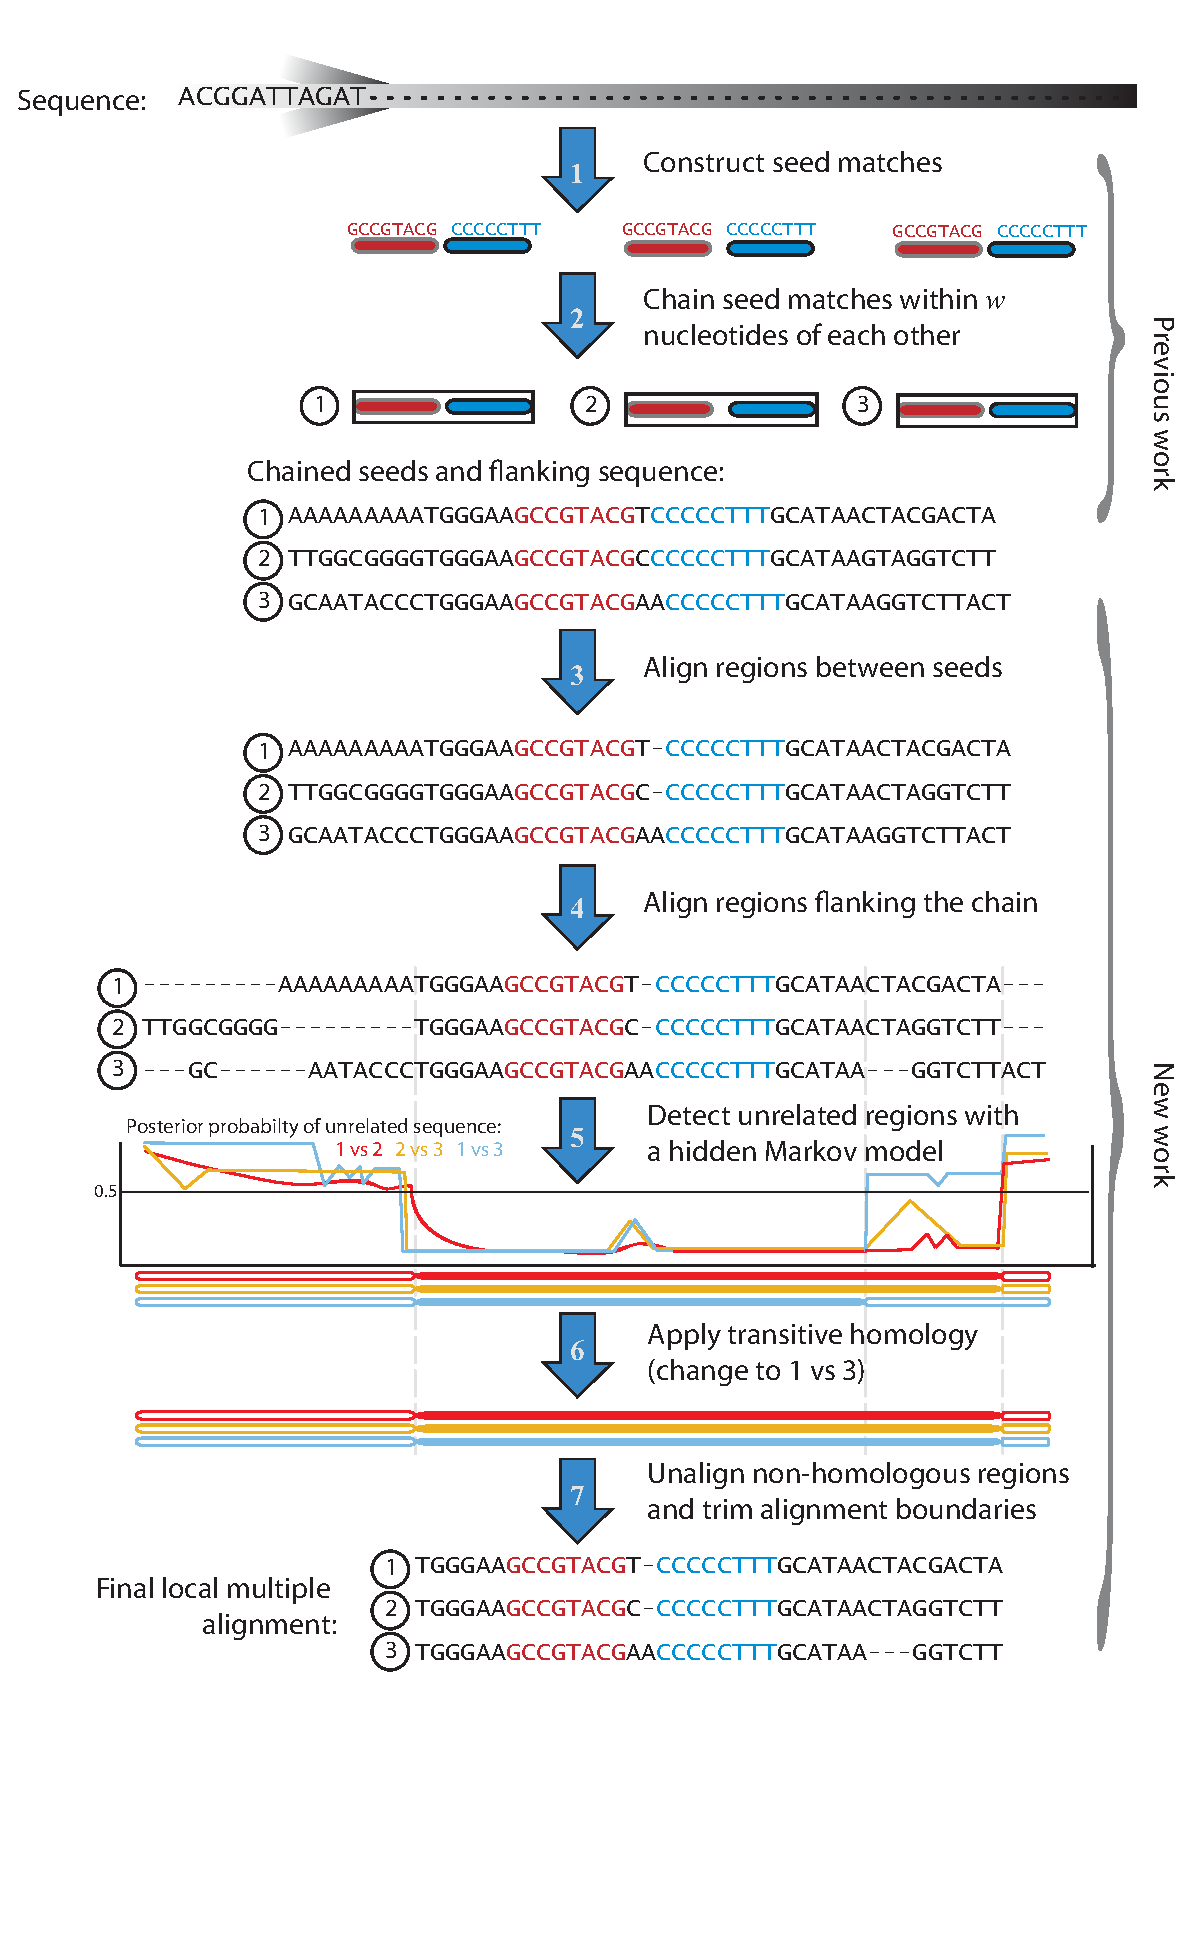
\epsfig{file=./figures/extension.eps,width=3.2in}}
\subfigure[Flowchart]{ 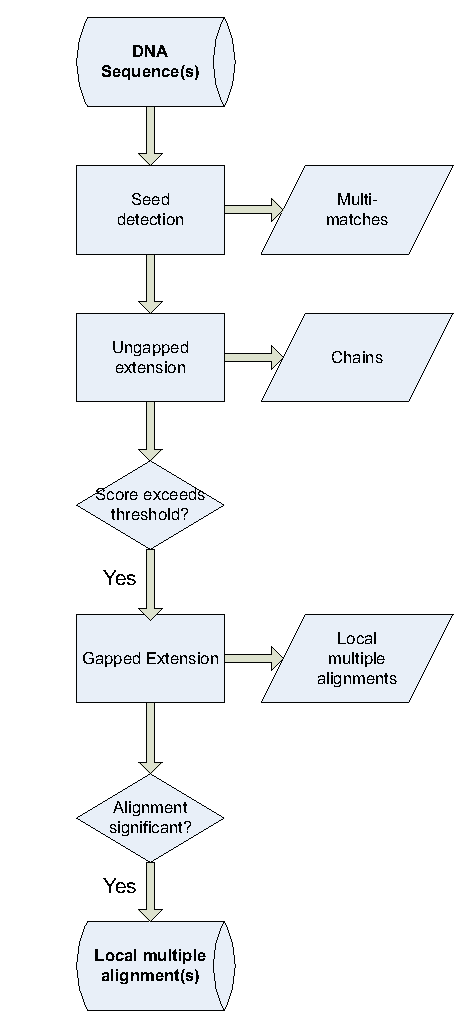
\epsfig{file=./figures/flowchart.eps,width=1.39in}}
\end{center}
\caption{Overview of the method}
\end{figure}


%\colorbox[named]{Gray}{adfa}

\subsection{Detecting seeds using a palindromic seed patterns}

As a starting point for homology detection, we locate all spaced seeds of a given weight $z$ in the input sequence(s). The palindromic spaced seed pattern is analyzed at each position in the input sequence to identify all multi-matches.  Previously we have demonstrated that palindromic spaced seeds offer good efficiency and sensitivity on a variety of input sequences~\cite{ref-procrast}. 

\subsection{Creating chains of multi-matches}

Once we have generated a list of multi-matches, we rely on our previously described method for efficient filtration method for maximal extension and chaining~\cite{ref-procrast}. 


\subsection{Gapped extension of all chains}
We would like to perform gapped
extension to detect all surrounding homologous sequence. Finding boundaries of sequence homology is a difficult and unsolved problem. We here present a novel heuristic for estimating boundaries of sequence homology, and we are very meticulous to avoid classify non-homologous DNA positions as homologous.


\subsubsection{Gapped alignment via MUSCLE}
We employ MUSCLE to perform gapped alignment in the regions surrounding the chains. We try extending 4*w nucleotides to the left/right of each chain. However, we only trigger gapped alignment if chain is above some minimum score threshold. This idea has been used in other local multiple alignment heuristics in order to minimize the number of gapped extensions that do not improve the boundaries of the chain. We score the resulting gapped alignment via sum of pairs. We continue to perform gapped alignment to the left/right) until we reach a score(calculated by sum of pairs) that has been previously determined via simulations to be non-homologous. i.e. a record height in the score signals the start of a stretch of non-homologous sequence.  If we improve our original seed boundaries we then trigger another round of extension, else we stop. 

\subsection{Calculating borders with random walk statistics}

\subsubsection{Random walk to extend homology border}
FIXME
\begin{itemize}
\item after scoring each column of the gapped extension, we would like
to determine where the homology ends/begins in this region
\item we do this by performing a random walk of the cumulative column score
\item we stop when we reach the record height
\item we determine the record height by simulations
\item all high scoring segments in the gapped extension are reported
\item if boundaries of the original chain are improved, trigger another round of extension.
\end{itemize}

\subsubsection{Processing Novel homologous sequence}
\begin{itemize}
\item novel homologous sequence can be found during gapped extension
\item should briefly describe what we do with this
\end{itemize}
\subsection{Unaligning non-homologous sequence}
FIXME
\begin{itemize}
\item our extension is not quite finished yet. Everything ok so far except that we could
still be including non-homologous sequence in our extended chain(local multiple alignment).
\item Define sets/subsets/boundaries with a pairwise homology test
\item first, we unalign any non-homolgous sequence introduced during the extension process
\item then, we define common boundaries among all sequences in the alignment
\end{itemize}



Ideally, once our algorithm finishes we will have a complete listing of all homologous local mulitple alignments. This list could be potentially overwhelming, and even at this point, we still need a way of selecting only the highly significant alignments. 

Finally, we would like to extend blast statistics to multiple local alignment. How?
\begin{itemize}
\item Extending Repseek simulations to multiple
\item Tompa et al, estimating the parameters for multiple alignments
\item will involve running procrastAlign with fixed parameters on sequences varying in composition and length
\item also will have to take into account multiplicity
\item FIXME: fill in more details on Monday
\end{itemize}

\section{Results}
We have created a program called \texttt{procrastAligner} for Linux,
Windows, and Mac OS X that implements the described algorithm. Our
open-source implementation is available as C++ source code licensed
under the GPL.


\subsection{Comparison with previous version of procrastAligner I}
\begin{table}[t]
  \centering
\begin{tabular}{lccccccccccc}
\hline Accession & Length & Rep & Family & Alu (bp) & Div, \% & Method & Sn \% & Sp \% & T (s) & Sw & $w$ \\
\hline
\hline AF435921 &  22 Kb &  28 & 10 & 261 (69) & 15.0 (6.4) & procrast & 100 & 95.9 & 1 & 9 & 27 \\
\cline{7-12}                                            &&&&&& procrastII & 100 & 97.0 & - & 9 & 27 \\
\hline Z15025 &    38 Kb &  52 & 13 & 245 (85) & 15.7 (5.7) & procrast & 100 & 82.5 & 2 & 9 & 27 \\
\cline{7-12}                                            &&&&&& procrastII & 100 & 77.5 & - & 9 & 27 \\
\hline AC034110 & 167 Kb &  87 & 18 & 261 (72) & 12.2 (5.9) & procrast & 100 & 97.9 & 3 & 15 & 45\\
\cline{7-12}                                            &&&&&& procrastII & 100 & 99.7 &- & 15 & 45 \\



\end{tabular}
\vspace{0.1cm}
  \caption{Performance of \texttt{procrastAlign}, and  \texttt{procrastAlignII} on Alu repeats.
  Rep: total number of Alu elements; Family: number of Alu
  families; Alu: average Alu length in bp (S.D.); Div: average Alu divergence (S.D.);
   Sn: sensitivity; Sp: specificity; T: compute time; Sw: palindromic seed weight; $w$: max gap size.  Alus were
  identified by RepeatMasker~\cite{ref-repbase}.}
  \label{table:alu}
\end{table}

 \subsection{Comparison with RepeatScount}

RepeatScout generates a repeat family consensus for all high frequency kmers via ungapped extension. As output, RepeatScout returns all families atleast 50nt long and occuring atleast 3 times in the input sequence(s). Once finished, RepeatScout uses RepeatMasker to locate all occurences of the repeat family in the input sequence(s).

How can we compare this to procrastAligner? 


\section{Discussion}

\subsection{Comparison of gapped
extension approaches}


\begin{itemize}

\item RepeatScout extends one nucleotide at a time
\item ABA merges pairwise matches and resolves inconsistencies by
whorl and bulge removal
\item multiz? and HomologMiner? also merge pairwise matches, how do
they resolve inconsistency?
\item procrastAligner generates multiple alignments using libMUSCLE,
which does progressive multiple alignment.  Progressive means that
pairwise alignments do enter in at some stage, but for higher
multiplicity matches, much of the alignment is multiple alignment.
cite a paper which shows multiple alignment is more accurate than
pairwise alignment.  MUSCLE's iterative refinement procedure ensures
a high-scoring alignment irrespective of guide tree.

\end{itemize}

\section{ Acknowledgments }
AED was supported by NLM Training Grant 5T15LM007359-05. TJT was
supported by Spanish Ministry MECD Grant TIN2004-03382 and AGAUR
Training Grant FI-IQUC-2005.

\bibliographystyle{splncs}
\small
\bibliography{procrastination}


\end{document}
